\documentclass[12pt,a4paper,oneside,openany,parskip=full,parindent=full]{book}
\usepackage[T1]{fontenc}
\usepackage[utf8]{inputenc}
\usepackage[polish]{babel}
\usepackage{graphicx}
\usepackage{times}
\usepackage{indentfirst}
\usepackage[left=3cm,right=2cm,top=2.5cm,bottom=2.5cm]{geometry}
\usepackage{natbib}
\usepackage{color}
\usepackage{tikz}
\usepackage{url}
\usepackage{dirtree}
\edef\restoreparindent{\parindent=\the\parindent\relax}
\usepackage{parskip}
\restoreparindent
\usepackage{listings}
\usepackage{enumerate}
\usepackage{color}
\usepackage{url}
\usepackage[hidelinks]{hyperref}

\definecolor{dkgreen}{rgb}{0,0.6,0}
\definecolor{gray}{rgb}{0.5,0.5,0.5}
\definecolor{mauve}{rgb}{0.58,0,0.82}

\lstset{frame=tb,
  language=Python,
  aboveskip=3mm,
  belowskip=3mm,
  showstringspaces=false,
  columns=flexible,
  basicstyle={\small\ttfamily},
  numbers=none,
  numberstyle=\tiny\color{gray},
  keywordstyle=\color{blue},
  commentstyle=\color{dkgreen},
  stringstyle=\color{mauve},
  breaklines=true,
  breakatwhitespace=true,
  tabsize=3
}


\frenchspacing
\linespread{1.5}
\addto\captionspolish{%
\renewcommand*\listtablename{Spis tabel}
\renewcommand*\tablename{Tabela}
}

\frenchspacing

\begin{document}

\begin{center}

\vspace{1cm}

Studium licencjackie
\end{center}

\vspace{1cm}

\noindent Kierunek: Informatyka

\noindent Specjalność: Bazy danych i technologie internetowe

\vspace{1cm}

{
\leftskip=10cm\noindent
Michał Polakowski\newline
Nr albumu: 203446\newline
Karol Chmielewski\newline
Nr albumu: 246668\newline
Michał Pydyszewski\newline
Nr albumu: 246631\newline
Bartłomiej Pysiak\newline
Nr albumu: 251191
}

\vspace{2cm}

\title{Praktyczne zastosowanie web scrapingu do tworzenia użytkowych aplikacji internetowych}
\makeatletter

\begin{center}
\LARGE\bf
\@title
\end{center}

\vspace{2cm}

{
\leftskip=10cm\noindent
Praca licencjacka\newline 
napisana w~Instytucie Matematyki, Fizyki i Informatyki\newline
pod kierunkiem naukowym\newline
dra Włodzimierza Bzyla

}

\vfill

\begin{center}
Gdańsk, \the\year
\end{center}
\thispagestyle{empty}

\clearpage
\thispagestyle{empty}
\clearpage

\tableofcontents

\clearpage
\chapter*{Streszczenie}

Nasza praca opisuje aplikację webową służącą jako pomoc w dopasowaniu za pomocą web-scrapingu elementu garderoby do najlepszych propozycji dostępnych w sklepach internetowych. 

Naszym celem było ukazanie w jaki sposób można zaimplementować web-scraping w aplikacji internetowej.

Web-scraping oparty jest na frameworku Scrapy, aplikacja zbudowana jest przy użyciu frameworka webowego Django, anonimizacja użytkownika i optymalizacja wydajnościowa jest możliwa dzięki serwerowi NGINX. Wszystkie zadania są obsługiwane przy użyciu kolejek dzięki Celery, a zbierane informacje są zapisywane w MongoDB oraz PostgreSQL. W pracy opisujemy działanie każdego z modułów, oraz przedstawiamy moralne aspekty web-scrapingu.
\chapter{Wprowadzenie}

Pomysł na naszą aplikację narodził się podczas odbywanych przez nas licznych wizyt w galeriach handlowych, gdzie zauważyliśmy jak dużo czasu, wysiłku i pieniędzy ludzie poświęcająm aby do posiadanej odzieży dopasować nowe elementy garderoby.

Na taki stan rzeczy składa się kilka czynników. Pierwszym z nich jest dostępność produktów. Wybór konsumenta ograniczony jest przez wyposażenie sklepów na terenie galerii. Ponadto, konsument ma tendencję do kupienia produktu, który w jego mniemaniu jest nabliższy temu, czego oczekiwał, lecz często nie dokładnie taki. To pokazuje nam kolejny problem - konsument nie pożytkuje swoich pieniędzy najlepiej, jak to możliwe. Nie sposób jest porównać wszystkich przedmiotów z puli potencjalnych dopasowań, ponieważ są one rozproszone po różnych sklepach, często galeriach, a nawet miastach. 

Trzecim czynnikiem jest czas poświęcony na wybieraniu potencjalnych dopasowań, ponieważ koniecznym jest fizycznie udać się do sklepów.

Jednym z rozwiązań problemu braku czasu jest zatrudnienie stylisty, który podpowie, które dopasowanie jest najlepsze, lecz jest to kosztowna usługa, na którą nie każdy może sobie pozwolić.

Odpowiedzią na te problemy jest nasza aplikacja. Po wprowadzeniu w pasku wyszukiwarki produktu, prezentowana jest użytkownikowi lista najlepiej skomponowanych do niego artykułów wraz z linkiem do sklepu, zdjęciem oraz ceną.
Wystąpienie na liście propozycji dopasowania podyktowane jest jego popularnością oraz częstotliwością doboru wśród innych użytkowników systemu.
Pozwala to na oszczędzenie czasu poprzez możliwość porównania bez wychodzenia z domu.
Aplikacja przyczynia się również do oszczędności pieniędzy, ponieważ niejako eliminuje potrzebę zatrudniania stylisty.

Produkt działa z wykorzystaniem web-scrapingu opartego na pythonowym frameworku Scrapy.
Poniższy diagram przedstawia po krótce proces działania wspomnianego modułu.

\begin{figure}[h]
    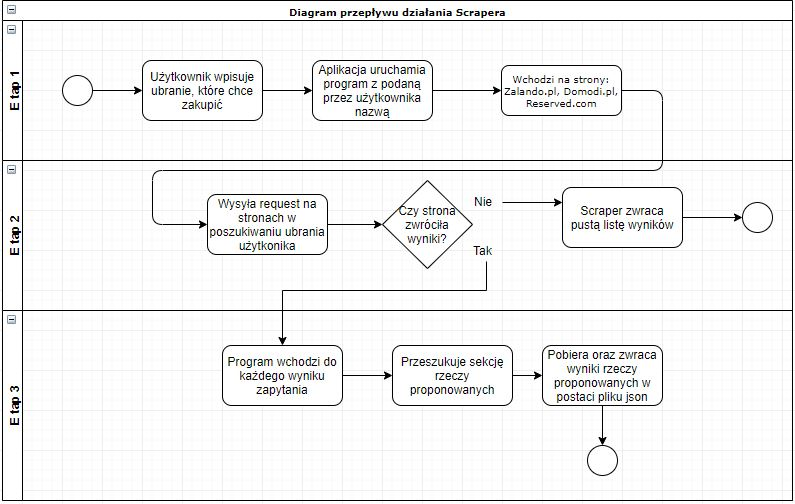
\includegraphics[width=1.1\textwidth]{zdjecia/diagram}
    \caption{Diagram działania scrapera. Wykonanie własne}
\end{figure}

Wyszukiwania są cachowane na serwerze pośredniczącym, co pozwala użytkownikowi na szybsze wyszukiwanie i płynniejsze korzystanie z aplikacji.
Zasoby statyczne takie jak zdjęcia pobierane są z serwera pośredniczącego, a nie z domeny docelowej.

Dodatkowym atutem korzystania z serwera pośredniczącego jest ukrycie prawdziwego adresu logicznego użytkownika, dzięki czemu utrudni to reklamodawcom prezentowanie mu reklam, co miałoby miejsce w przypadku bezpośrednich wizyt w poszczególnych domenach sklepów internetowych.sklepach

W projekcie wykorzystujemy load balancing, dzięki któremu ruch będzie rozpraszany na wszystkie węzły, a użytkownik nie odczuje spadku wydajnośći w przypadku wzmożonego ruchu.

\textbf{Słowa kluczowe:} web-scraping, dopasowanie ubrań, stylizacja modowa
\chapter{Django}

Python jest aktualnie jednym z najpopularnijeszych języków programowania na świecie, a co za tym idzie liczba frameworków, które się na nim opierają jest dość pokaźna. Nasz wybór w kwestii obsługi backendu aplikacji padł na Django z kilku powodów, które chciałbym w tym rozdziale pokrótce przedstawić. 

\section{Popularność}
Pierwszym czynnikiem wpływającym na nasz wybór była popularność frameworka. Django bez wątpienia jest jednym z najczęściej używanych pythonowych narzędzi do obsługi serwerowej strony aplikacji internetowych. Oprócz popularności wśród pythonowych frameworków jest on niewątpliwie również jednym z njaczęściej wybieranych w ogóle. Na jego popularność z pewnością wpływa podejście "batteries included", to znaczy koncepcja frameworka, który najważniejsze elementy współczesnych aplikacji internetowych ma niejako wbudowane. Możliwość obsługi frontendu poprzez wbudowany system template'ów, formularze tworzone bezpośrednio po stronie django i w prosty sposób renderowane na froncie, czy system autentykacji, który praktycznie nie wymaga modyfikacji (chyba, że ich potrzebujemy) - to wszystko również kierowało milionami użytkowników przy wyborze tego narzędzia do budowy ich projektów. 

Z pewnością początki Django sięgające okolic 2006 roku pozwoliły na uformowanie się bardzo dużej społeczności, która sukcesywnie budowała, i wciąż buduje niezliczone ilości narzędzi wspomagających proces tworzenia i obsługi kolejnych aplikacji internetowych.

\section{Modularność}
Wymieniając w pierwszej części tego rozdziału powody popularności obiektu naszego zainteresowania, siłą rzeczy zahaczyłem również o powody, dla których Django stało się naszym wyborem jako silnik backendu budowanej przez nas aplikacji. Jednym z nich jest właśnie jego modularność - aspekt, który jest niejako bezpośrednią konsekwencją popularności. Mianowicie przez słowo modularność mam na myśli technikę budowania systemów, która kładzie nacisk na podzielenie poszczególnych funkcji programu w niezależne, wymienne moduły w taki sposób, aby dana funkcja mogła być w pełni wykonana przez dany moduł.

Modularność Django można zauważyć w kilku aspektach: 

\subsection{Jedna funkcjonalość, jedna aplikacja}
Przy tworzeniu podstawowego schematu djangowej aplikacji zauważyć można, że cli frameworka tworzy strukturę folderów zbliżoną do następującej
\dirtree{%
.1 projectname.
.2 projectname.
.3 settings.py.
.3 urls.py.
.3 wsgi.py.
.2 app1.
.3 models.py.
.3 views.py.
.2 app2.
.3 models.py.
.3 views.py.
}

Pokazuję oczywiście jedynie najważniejsze z technicznego punktu widzenia pliki.\cite{Dokument39:online} Założeniem frameworka jest wyabstrahowanie każdej funkcjonalności aplikacji do oddzielnych folderów (na schemacie: app1, app2). Każdy z nich powinien zawierać oddzielne modele oraz widoki stricte odnoszące się do danej części budowanego systemu. Pozwala to na łatwe przyłączanie kolejnych, nowych elementów do gotowej aplikacji, a także tworzenie modułów wielokrotnego użytku.

\subsection{Gotowe paczki}
W związku z liczną społecznością zgromadzoną wokół Django bez większych problemów możemy znaleźć gotowe rozwiązania napotkanych problemów czy uzupełnienia frameworka o funkcjonalności, których wprowadzenia do rdzenia nie przewidzieli twórcy. Jednym z największych tego typu rozwiązań jest Django Rest Framework - narzędzie służące do budowy API w stylu architektury REST.

\subsection{Bierz co chcesz}
Przede wszystkim już w samym kodzie frameworka znaleźć możemy moduły, które możemy, choć wcale nie musimy wykorzystać. Wspomniany juz w tym rozdziale moduł autentykacji zawiera podstawowe modele użytkownika naszego systemu, formularze rejestracji i logowania, a nawet wbudowane widoki odzyskiwania hasła.Nie ma żadnego przymusu korzystania z nich, jednak mało która apliakcji webowa nie korzysta z tego typu funkcjonalności. Sprawa ulega komplikacji, gdy wbudowane funkcjonalności nie odpowiadają w pełni naszym potrzebom, jednak z Django nie stanowi to większego problemu - nadpisywanie, dopisywanie i ogólna modyfikacja gotowych elementów jest intuicyjna i szybka.

\section{ORM}
Jednym z elementów, który wyróżnia Django jest jego ORM:
\begin{lstlisting}
from django import models

class AuthorModel(models.Model):
	name = models.CharField('Name', max_length=50)

class BookModel(models.Model):
	title = models.CharField('Title', max_length=100)
	author - models.ForeignKey(Author, on_delete=models.CASCADE)
	
\end{lstlisting}

Przedstawiony fragment kodu przedstawia reprezentację schematu tabel zawierających dane na temat książek i ich autorów. Atrybuty klasy definiują kolumny i ich typy.\cite{djangobestpractices} 
Taki sposób planowania bazy danych pozwala na niemal obrazowe przedstawianie jej przyszłej budowy, a także zwiększa czytelność zależności wystepujących między poszczególnym encjami naszej aplikacji.Obsługa wielu różnych baz danych jest wspierana dzięki paczkom przygotowanym przez społeczność. 
\chapter {Moduł Bramy}

Moduł bramy ma za zadanie optymalizację i dystrybucję ruchu sieciowego.
Używa NGINX jako serwera pośredniczącego aby zapewnić możliwie najkrótszy czas
odpowiedzi dla użytkownika aplikacji.

W związku z tym możemy wyszczególnić 5 głowne zadania, jakie serwer bramy wykonuje:


\begin{itemize}
  \item Load balancing
  \item Cachowanie
  \item Anonimizacja użytkownika
  \item Zwiększenie wydajności
  \item Skalowalność
\end{itemize}

\section{Load balancing}

Load balancing to technika redukowania obciążenia wynikającego z ilości zapytań jakie serwer musi obsłużyć poprzez dystrybuowanie ruchu na więcej niż jedną instancję, która jest w stanie takie zapytania obsłużyć. Nasz system musi zapewniać użytkownikowi poczucie lekkości niezależnie od ilości aktualnie nawiązanych połączeń. Aby rzeczywiście znalezienie najlepszego dla wybranej rzeczy dopasowania wiązało się z oszczędnością czasu, z perspektywy infrastruktury musimy zapewnić możliwie najkrótszy czas odpowiedzi.
Na serwerze bramy do dystrybucji ruchu wybrany został algorytm karuzelowy - wszystkie procesy mają ten sam priorytet.
\begin{lstlisting}
  http {
    upstream app1 {
      server srv1.example.com
      server srv1.example.com
      server srv1.example.com
    }
  }
\end{lstlisting}

\section{Caching}

Funkcjonalność aplikacji oraz korzyści jakie daje ona użytkownikowi opierają się między innymi na możliwości szybkiego porównania i wyciągnięcia wniosków dotyczących potencjalnego dopasowania. Możliwe jest to dzięki wyświetleniu zdjęcia znalezionego produktu. Nieżadko może się zdażyć, że propozycje dopasowań będą się powtarzać. Daje to możliwość cachowania plików statycznych, dzięki czemu kolejne rządanie HTTP po taki zasób będzie serwowane bezpośrednio z dysku twardego serwera bramy, a nie z serwera docelowego.
Co więcej, NGINX daje udostępnia interfejs do ustawienia cachowania po stronie klienta, dzięki czemu zasoby statyczne w razie rządania HTTP będą pobierane bezpośrednio z pamięci podręcznej przeglądarki.

\begin{lstlisting}
  location ~* \.(jpg|jpg|png|gif|ico)$$ {
    expires 30d;
  }
  
  location ~* \.(css|js)$$ {
    expires 7d;
  }
\end{lstlisting}

\section{Anonimizacja}
Niezbędnym jest zapewnienie bezpieczeństwa użytkownika i systemu.
Bezpieczeństo użytkownika jest rozumiane przez nas jako anonimizacja jego wyszukiwań. W przypadku korzystania z NGINX jako serwera pośredniczącego anonimizacja wynika naturalnie z architektury systemu.
Rządania HTTP po zasoby udostępniane przez sklepy internetowe są wykonywane z adresem logicznym bramy, a nie użytkownika końcowego.
Dzięki temu sklepy pozbawione są możliwości targetowania reklam dla użytkownika  biorąc pod uwagę jego poprzednie wizyty. Dzięki temu użytkownikowi aplikacji nie będą prezentowane reklamy powiązane z wyszukiwanym produktem - nie zapewniają one w żaden sposób, że reklamy będą dotyczyć rzeczy pasujących, a jedynie podobnych, lub nawet tych samych.

\section{Zwiększenie wydajności}
Pośród ogromu możliwości, jakie serwer NGINX daje w kontekście optymalizacji ruchu, wybraliśmy kilka, które w najbardziej bezpośredni sposób wpływają na wydajność naszej infrastruktury:

\begin{enumerate}
\item
Ustawienie liczby procesów potomnych serwera na podstawie liczby CPU oraz dysków twardych
\begin{lstlisting}
worker_processes auto;
\end{lstlisting}
\item
Zwiększenie liczby operacji weścia/wyjścia na dysku twardym przez wyłączenie logowania
\begin{lstlisting}
error_log /var/log/nginx/error.log crit;
access_log off;
\end{lstlisting}
\item
Wymuszenie na  wysłania danych z bufora tak szybko jak to możliwe, pomijając algorytm Nagle'a, według którego pakiet, który jest za mały, czeka według standardowej implementacji UNIX 200 milisekund na wypełnienie.
\begin{lstlisting}
tcp_nodelay on;
\end{lstlisting}
Wymuszenie na pakiecie blokady zanim osiągnie maksymalny rozmiar
\begin{lstlisting}
tcp_nopush on;
\end{lstlisting}
\end{enumerate}

\section{Skalowalność}
Wraz ze wzrostem zainteresowania systemem, musimy przewidzieć, że w pewnym momencie obecna architektura może nie być wystarczająca, aby zapewnić stabilność i wysoką wydajność. Serwer NGINX jest zorientowany wokół jednego procesu głównego i wielu procesów potomnych zależnie od liczby rdzeni CPU i dysków twardych. W miarę potrzeby możemy zwiększyć liczbę rdzeni procesora, a przez to zwiększyć też liczbę procesów potomnych.
Infrastruktura jest zorientowana zarówno wokół konieczności skalowalności wertykalnej, ale również horyzontalnej. Zwiększenie liczby procesów na które dystrybuowany jest ruch w procesie load-balancingu również jest możliwe i zapewni stabilność w przypadku potrzeby skalowania.




\chapter {Scraper} 

W niniejszym rozdziale zajmę się omówieniem użytych w projekcie zagadnień dotyczących webscrapingu.

Scrapy jest jedną z najpopularniejszych bibliotek pythonowych, które mają za zadanie zbierać informacje ze stron internetowych.
Webscraping oparty jest na pyhtonowym frameworku \emph{Scrapy}, wspieranym przez biblioteki \emph{Splash} oraz \emph{XPath}.
Uzyskiwałem wiedzę posługując się dokumentacjami bibliotek \emph{Scrapy}\footnote{\url{https://doc.scrapy.org}}, \emph{Splash}\footnote{\url{https://splash.readthedocs.io/en/stable/api.html}} oraz \emph{XPath}\footnote{\url{https://doc.scrapy.org/en/xpath-tutorial/topics/xpath-tutorial.html}}.

Skrypt uruchamiany jest na trzech stronach sklepów internetowych: \emph{https://reserved.com, https://zalando.pl, https://domodi.pl}. 
Wykonywanie programu jest podzielone na trzy etapy:
\begin{enumerate}
	\item Po uzyskaniu słów kluczowych program wprowadza w wyszukiwarce strony daną frazę wpisaną przez użytkownika.
	\item Przekierowuje do wszystkich wyników wyszukiwania.
	\item Zbiera oraz zwraca informację z rubryki wygenerowanej dynamicznie przez stronę, która	ma na celu poinformowanie kupującego o rzeczach zakupionych przez innych użytkowników wraz z wyszukiwanym ubraniem.
\end{enumerate}
\section{Opis etapów}

\subsection{Etap 1}
	Aplikacja włącza program scrapingowy za pomocą następującej komendy: \emph{scrapy crawl clothing -a tag=”fraza” -o results.json}.
Oznacza to uruchomienie programu o nazwie \emph{clothing} z parametrem do wyszukania (tag), a rezultat będzie przechowywany do pliku \emph{results.json}.
Po uruchomieniu, do każdej strony internetowej inicjowana jest metoda \emph{search}, która za pomocą \emph{XPath} odszukuje formularz na stronie głównej sklepu, wpisuje interesującą użytkownika nazwę ubrania i wysyła request z żądaniem wyszukania.

\subsection{Etap 2}
	Strona sklepu internetowego zwraca wyniki wyszukiwania. Program zbiera wszystkie linki do wyszukanych ubrań za pomocą \emph{XPath}, który przeszukuje w kodzie HTML odnośniki mające w adresie przekierowującym rodzaj ubrania. Następnie przechodzi do tych stron odpalając kolejną metodę, która zależnie od sklepu szuka w kodzie HTML strony innych struktur.

\subsection{Etap 3}
	Będąc na tym etapie program jest już w dokładnie jednej ofercie zakupu ubrania. Zależnie od strony, skrypt zachowuje się w inny sposób:
\begin{itemize}
	 \item dla stron \emph{reserved} oraz \emph{domodi} od razu następuje przeszukiwanie kodu HTML w celu znalezienia proponowanych rzeczy poprzez znalezienie odpowiedniej struktury
		\begin{itemize} 
			\item dla sklepu Reserved każda oferta przeszukiwania jest umieszczona w znaczniku \textless div\textgreater, a znacznik ten zaczyna się od klasy, która ma nazwę \emph{portrait}. Dla Domodi jest to każdy 	znacznik \textless li\textgreater.
		\end{itemize}
	\item dla sklepu Zalando wyszukiwany jest najpierw tekst \emph{zobacz więcej}. Po znalezieniu tekstu aplikacja przechodzi na tą podstronę, żeby móc wylistować wszystkie ubrania proponowane przez sklep. W przypadku, gdy tekst \emph{zobacz więcej} nie zostanie znaleziony, aplikacja nie zwróci żadnych propozycji ze strony Zalando.\end{itemize}
Program pobiera następujące informacje z propozycji kupna:
\begin{itemize}
	\item adres URL
	\item zdjęcie ubrania
	\item cenę
	\item nazwę ubrania
\end{itemize}
Informacje zapisywane są tylko wtedy, jeśli jest ich cały komplet – powoduje to uniknięcie przedostawania się do wyników niepotrzebnych danych bądź innych przypadkowo pobranych rzeczy.
Zapisywanie odbywa się w formacie json o strukturze słownikowej:
\begin{itemize}
\item[] \emph{\{ClothesName: \{ "image": imageURL, "price": PRICE, "url": URL\}\}}
\item[] \emph{ClothesName} – przechowywany w formacie string; jako wartość zawiera słownik ze szczegółami
\item[] \emph{imageURL} – przechowywany w formacie string; zawiera adres do zdjęcia ubrania
\item[] \emph{PRICE} – przechowywany w formacie string; zależnie od strony może być z końcówką „zł” lub „PLN”
\item[] \emph{URL} – przechowywany w formacie string; zawiera adres do strony sklepu z daną rzeczą
\end{itemize}
Program na bieżąco przesyła taki słownik do pliku wynikowego, z którego dalsza część programu może na bieżąco czytać.


Program, żeby mógł działać na dynamicznych stronach używa biblioteki Splash.
Splash używa funkcji napisanej w języku Lua:
\begin{lstlisting}
function main(splash, args)
          assert(splash:go(args.url))
          assert(splash:wait(0.5))
          assert(splash:set_viewport_full())
          return {
            html = splash:html()}
            end
\end{lstlisting}\footnote{\url{https://splash.readthedocs.io/en/stable/scripting-tutorial.html}
\begin{itemize}
\item[] Splash:go(args.url) przechodzi na stronę podaną w argumencie.
\item[] Splash:wait(0.5) – określa jak długo program czeka na załadowanie strony
\item[] Splash:set\_viewport\_full() sprawia, że wczytywana jest cała strona HTML

Wysyłanie requestów do stron również odbywa się za pomocą metody z biblioteki Splash -- \emph{SplashRequest}, która jako argumenty przyjmuje adres strony, metodę do której ma przejść w następnym kroku oraz argumenty (przekazanie całej funkcji z języka Lua jako parametr).
\end{itemize}
\section{Dlaczego Scrapy}

Scrapy jest stosunkowo dużym frameworkiem skupionym na webscrapingu. Nie jest trudno opanować podstawy -- framework ten jest bardzo dobrze udokumentowany oraz posiada dużo poradników dotyczących pierwszych kroków. Wszystkie te udogonienia pozwalają poznać podstawowe fundamenty Scrapy, które w dużej mierze powinny wystarczyć do większości zadań związanych z webscrapingiem. Posiada własne selektory, dzięki którym można swobodnie poruszać się po stukturze HTML. Jego największą zaletą jest to, że służy jako crawler -- wystarczy podać adres początkowy, a framework będzie w stanie przeszukiwać wgłąb stronę wedle chęci osoby piszącej program.

Przy wielkości opisywanego przez nas projektu oraz przy daleko idących planach rozbudowy aplikacji pisanie crawlera we frameworku w pełni skupionym na scrapingu jest niezbędne do uniknięcia dalszych problemów związanych z obsługą coraz bardziej skomplikowanych stron internetowych.
\subsection{Selektory}

Scrapy implementuje własne selektory pozwalające przeszukiwanie kodu HTML.
Można wydobywać części kodu za pomocą języka XPath oraz poprzez wybieranie kodu CSS, który stylizuje HTML.

W opisywanej aplikacji zdecydowałem się na posługiwanie się językiem XPath -- był dla mnie wygodniejszy i łatwiejszy w nauce.
Przykładowy selektor z napisanego przeze mnie scrapera, który jest używany w naszym programie:
\begin{lstlisting}
response.xpath("//a[./img[contains(@src,.)]]/@href").extract()
\end{lstlisting}
Powyższa linijka oznacza wybranie wszystkich znaczników \textless a\textgreater. Następnym krokiem jest znalezienie takich znaczników \textless img\textgreater, które posiadają w sobie odnośniki do innych stron. 
\emph{Extract()} powoduje, że wszystkie wyniki wyszukiwania pojedynczo będą formatowane jako typ string, który będzie można przekształcić wedle uznania.
Ważnym elementem selektorów jest możliwość wyszukania danej informacji znajdującej się wewnątrz wybranych znaczników.
Za przykład posłuży mi fragment kodu. Ma on za zadanie zebrać wszystkie niezbędne informacje na temat strony \emph{zalando.pl}:
\begin{lstlisting}
        for item in response.xpath("//div[./a[contains(@href,'zalando.pl')]]"):
            url = item.xpath('./a/@href').extract()
            itemImg = item.xpath('.//*/img[contains(@src,.)]/@src').extract()
            price = item.xpath(".//span[contains(text(),'zl')]/text()").extract_first()
            itemName = item.xpath('.//*/img[contains(@src,.)]/@alt').extract()
\end{lstlisting}

Kod ten napisałem sam, za pomocą dokumentacji Xpath oraz Scrapy. Xpath zaczynający się od kropki oznacza, że program zaczyna przeszukiwać od -- podanego w przykładzie wyżej, \textless a\textgreater. Wybierane są tylko hiperłącza posiadające odnośnik do strony zawierającej podstring "zalando.pl".

Finalnie, jeśli zdajemy sobie sprawę które rzeczy Scrapy powinien szukać oraz mamy otwartą stronę z dokumentacją\footnote{\url{https://doc.scrapy.org}}, to napisanie owego crawlera od podstaw, nie znając wcześniej składni, okazuje się stosunkowo proste i przyjemne.

\chapter {Wizualna prezentacja projektu} 

Niniejszy rozdział poświęcony jest przedstawieniu projektu ze strony wizualnej.

Wchodząc na naszą aplikację pierwszym obrazkiem, który nas powita jest strona tytułowa wraz z zablokowanym oknem formularza, w którym będziemy mogli wpisać nazwę ubrania, do którego program będzie szukać dopasowań.

\begin{figure}[h]
    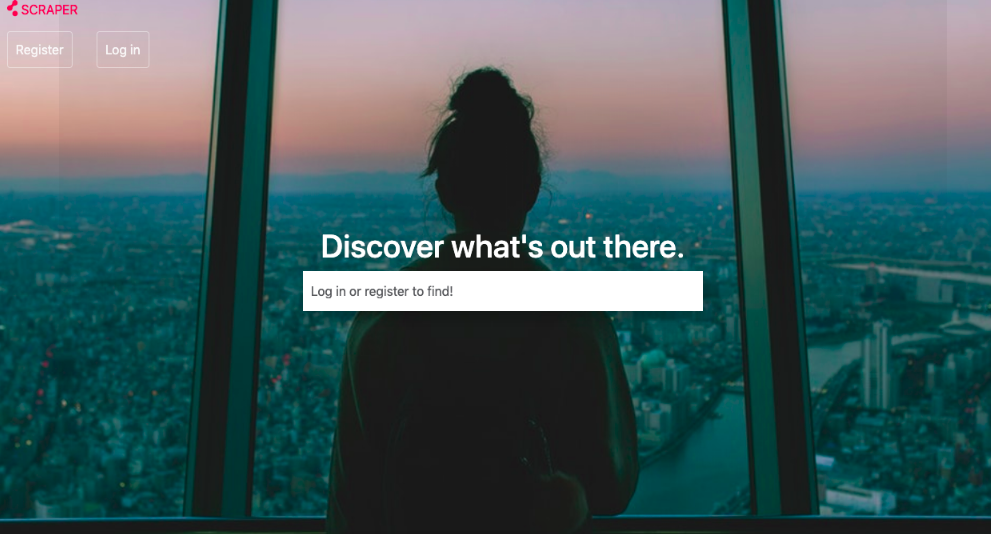
\includegraphics[width=1.10\textwidth]{zdjecia/tytulowa}
    \caption{Strona tytułowa}
\end{figure}

Użytkownik, żeby móc korzystać z aplikacji musi się zarejestrować. W tym celu klika przycisk \emph{Register}, a następnie wypełnia formularz.

\begin{figure}[h]
    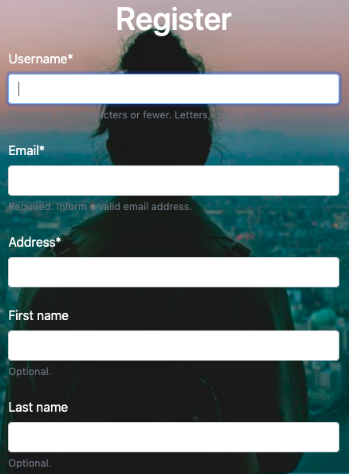
\includegraphics[height=10cm]{zdjecia/registration}
    \caption{Formularz rejestracji}
\end{figure}

\newpage
Następnym krokiem po rejestracji jest logowanie. Używając danych wpisanych podczas rejestracji można zalogować się do systemu.

Od tej chwili użytkownik może korzystać z aplikacji w stu procentach.\newline
Pojawiło się okna \emph{History} oraz \emph {Results}, w których odpowiednio można przeglądać swoją historię wyszukiwań oraz wyniki ostatniego wyszukania.
\begin{figure}[h]
    
\includegraphics{zdjecia/history_results}
    \caption{Wszystkie okna użytkownika}
\end{figure}

Jeśli przejdziemy do podstrony z historią wyszukiwań, otrzymamy widok z tabelą, która ma dwie kolumny: \emph{Name} i \emph{Date}.\newline
Tabela jest sortowalna, jest możliwość wyszukania na podstawie frazy wpisanej przez użytkownika.
\begin{figure}[h]
    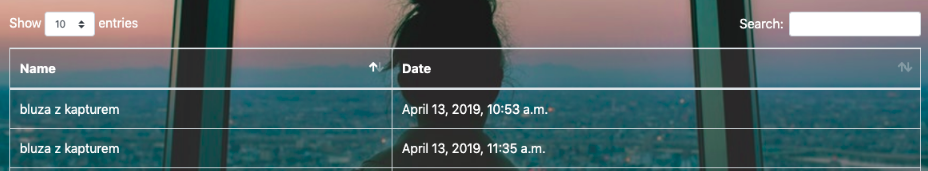
\includegraphics[width=1.10\textwidth]{zdjecia/history}
    \caption{Historia wyszukiwań}
\end{figure}
\newpage
Na stronie głównej zostało odblokowane okno z wyszukiwaniem. W tym celu można wpisać interesującą użytkownika rzecz, a następnie przejść do zakładki results, w której pojawi się tabela z nazwą ubrania, ceną, linkiem do sklepu oraz linkiem do zdjęcia. Tabela jest w pełni sortowalna, można wyszukiwać danej frazie.
\begin{figure}[h]
    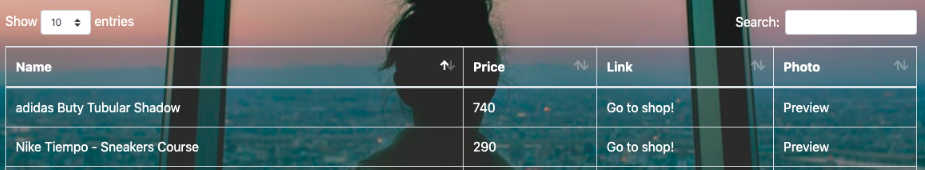
\includegraphics[width=1.10\textwidth]{zdjecia/wyniki}
    \caption{Wyniki wyszukiwań}
\end{figure}

\chapter{Etyczne i prawne aspekty web-scrapingu}

\section{Wprowadzenie}

	Web scraping ze względu na swoje działanie jak i późniejsze wykorzystywanie pozyskanych informacji traktowany jest zwykle jako procedura wątpliwa nie tylko moralnie, ale często również jako działanie nie do końca zgodne z prawem. Mamy tu przecież do czynienia z pozyskiwaniem, zwykle bez wiedzy właściciela strony, portalu czy serwisu, informacji, które mogą być objęte prawami autorskimi, naruszającymi czyjąś prywatność lub wręcz tajnymi (ale nie dostatecznie zabezpieczonymi).

\section{Scraping w życiu codziennym, regulacje prawne}

Podstawy prawne, które mogą regulować zasady działania web-scrapingu różnią się w zależności od naszego położenia na kuli ziemskiej. Ogólnie rzecz biorąc, takie wytyczne mogą być ujęte w zasadach korzystania z danej strony internetowej. Przestrzeganie tychże zasad i dochodzenie swoich praw ze strony „poszkodowanego” portalu nie zawsze jest jasne i łatwe do przeprowadzenia. Biorąc pod uwagę powyższe, niektóre kraje zdecydowały się wprowadzić regulacje, które wprost decydowałyby o tym, co jest, a co nie jest legalne. Jednakże, ze względu na różnorodność jaka charakteryzuje działania związane ze scrapingiem ostateczna decyzja należy zwykle do sądu. Mowa tu oczywiście o działaniach, których nie można wprost określić jako nielegalnych np. kradzieży danych i wykorzystywania ich w negatywnych celach. Spory kończące się na ławach sądowych dotyczą zwykle wielkich korporacji działających przede wszystkim w sieci takich jak Facebook, Google, LinkedIn, ale również firm działających w różnych gałęziach gospodarki, ale w obecnych czasach nierozerwalnie związanych już z Internetem. 
	
Ponieważ spraping wykorzystywany jest przez strony dzięki którym można na przykład porównywać ceny biletów lotniczych, sprawdzać dostępność hoteli, ceny pokoi czy chociażby porównywać ceny dostępnych produktów w bezmiarze sklepów internetowych istniejących obecnie. Z punktu widzenia konsumenta działania takie są jak najbardziej pozytywne, jednak z punktu widzenia sprzedawcy już nie tak bardzo. Te same dane, zamiast służyć dobru konsumenta, wykorzystane mogą być również przez inne firmy do nie do końca czystych zagrań, jak np. celowe obniżanie cen. 

Inny negatywny aspekt zauważyć można chociażby w przypadku odpłatnych imprez masowych. Dotyczy to zjawiska „automatycznego podkupowania” biletów przez inne podmioty oczywiście w celach uzyskania dodatkowych korzyści z późniejszej ich sprzedaży po swoich cenach. Aby temu przeciwdziałać wprowadzono ograniczenia w ilości kupowanych biletów przez pojedynczego użytkownika. Nie jest to rozwiązanie idealne, ale też nie uderza zbytnio w konsumenta zainteresowanego kupieniem biletu w najlepszej możliwej cenie. 

\section{Podsumowanie}

Scraping w różnych formach istniał praktycznie od momentu rozpowszechnienia się internetu i zapewne istniał będzie aż po jego kres (albo i dłużej). Biorąc pod uwagę zalety, które przynoszą takie działania ciężko stwierdzić czy zaistnieje kiedykolwiek wykładnia, która raz na zawsze zabroni jednym podmiotom korzystać z danych zamieszczanych w sieci przez innych. 

Jak pokazuje historia, każdy przypadek wchodzenia na drogę sądową przez firmy „dotknięte” działaniem scrapingu jest inny i bez ścisłych uregulowań prawnych nie do przewidzenia jest decyzja jaka zostanie podjęta przez sąd rozpatrujący daną sprawę. 
\chapter{Diagramy}

\section{Wprowadzenie}

W poniższym rozdziale przedstawione zostały diagramy sekwencji i klas opisujące tworzoną przez nas aplikację. 

Diagramy sekwencji przedstawiają zależności czasowe pomiędzy obiektami oraz służą do modelowania systemów czasu rzeczywistego i złożonych scenariuszy\footnote{\url{https://pl.wikipedia.org/wiki/Diagram_interakcji}}. Natomiast diagramy klas pokazują określony fragment struktury systemu. Diagramów klas używa się do modelowania statycznych aspektów perspektywy projektowej. Wiąże się z tym silnie modelowanie słownictwa systemu, kooperacji lub schematów. Diagramy klas pozwalają na sformalizowanie specyfikacji danych i metod. Mogą także pełnić rolę graficznego środka pokazującego szczegóły implementacji klas\footnote{\url{https://pl.wikipedia.org/wiki/Diagram_klas}}.
\newpage
\section{Diagram sekwencji}

\begin{figure}[h]
    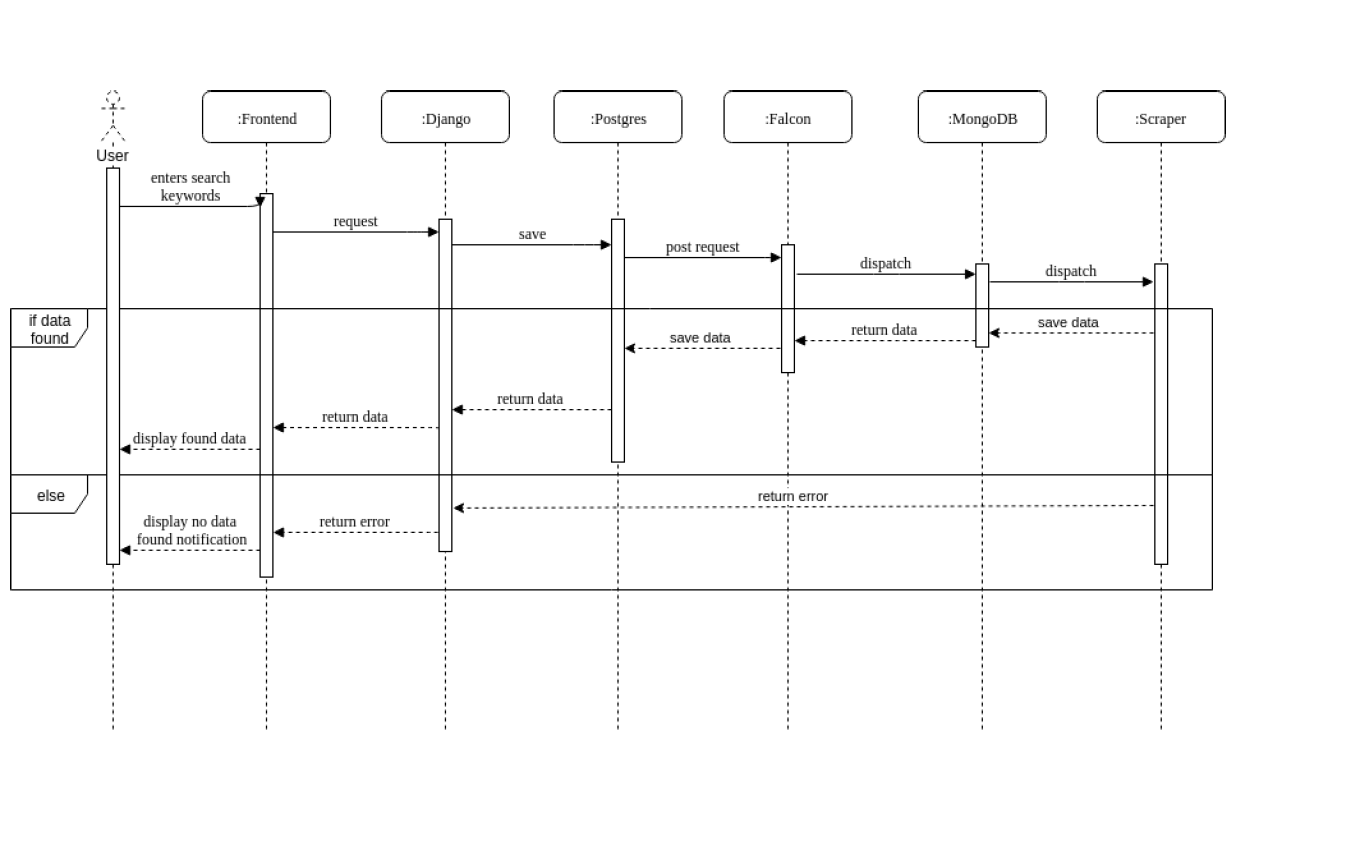
\includegraphics[width=1.10\textwidth]{zdjecia/sekwencja}
    \caption{Diagram sekwencji. Opracowanie własne}
\end{figure}
\newpage

\section{Diagram klas}

\begin{figure}[h]
    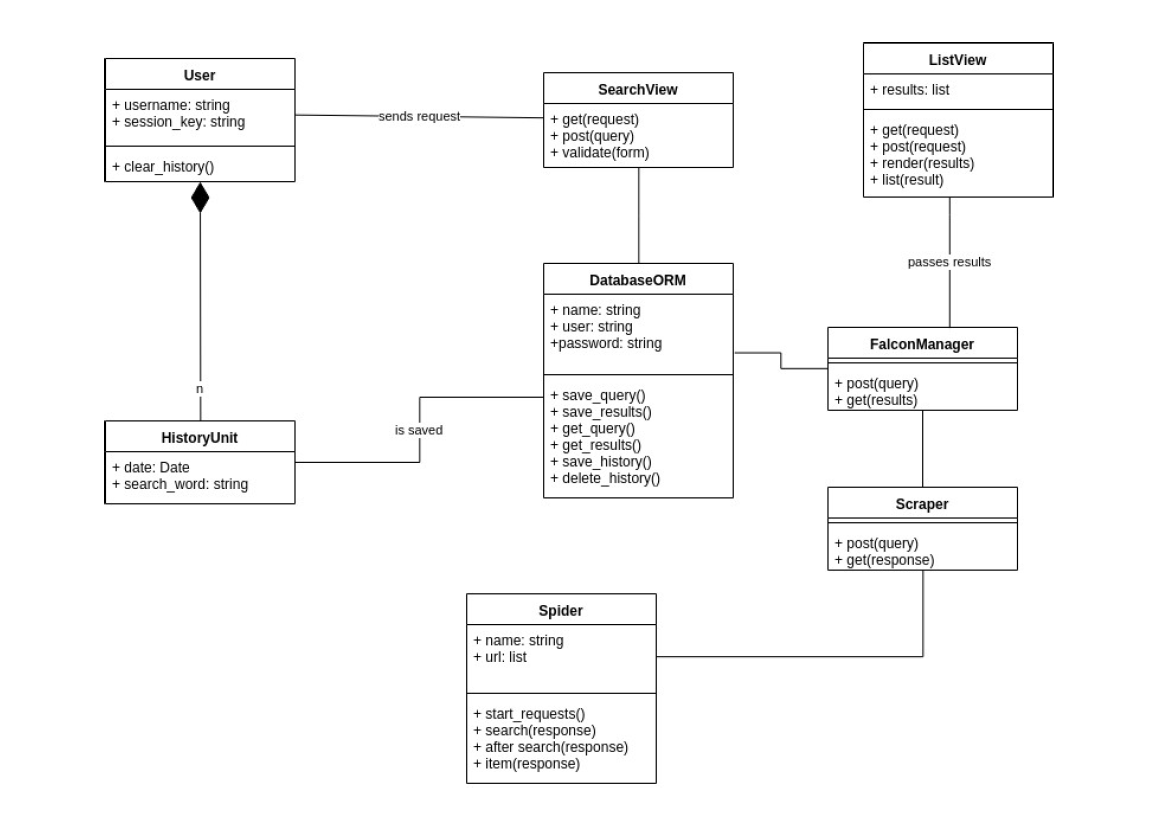
\includegraphics[width=1.10\textwidth]{zdjecia/klas}
    \caption{Diagram klas. Opracowanie własne}
\end{figure}




\bibliographystyle{plain}
\bibliography{bibliografia/main}

\clearpage


\end{document}
